\documentclass[a4paper,11pt,twoside,openright]{article}

\usepackage[toc,page]{appendix}
\usepackage{amsmath}
\usepackage{geometry}
\usepackage{graphicx}
\usepackage{subcaption}
\usepackage{multirow}
\usepackage[section]{placeins}
\usepackage{array}
\usepackage[nottoc,numbib]{tocbibind}
\usepackage{multicol}
\usepackage{wrapfig}
%\usepackage{titlesec}

\geometry{margin=1in}
\graphicspath{ {Images/} }

\newcolumntype{?}[1]{!{\vrule width #1}}
\newcommand{\Mod}[1]{\ (\mathrm{mod}\ #1)}

\let\oldsection\section
\def\section{\cleardoublepage\oldsection}

%\setcounter{tocdepth}{4}

%\titleformat{\paragraph}
%{\normalfont\normalsize\bfseries}{\theparagraph}{1em}{}
%\titlespacing*{\paragraph}
%{0pt}{3.25ex plus 1ex minus .2ex}{1.5ex plus .2ex}

\begin{document}

%%%%%%%%%%%%%%%%%%%%%%%%%%%%%%%%%%%%%%%%%%%%%%%%%%%%%%%%%%%%%%%%%%%%%%%%%%%%%%%
% TITLEPAGE                                                                   %
%%%%%%%%%%%%%%%%%%%%%%%%%%%%%%%%%%%%%%%%%%%%%%%%%%%%%%%%%%%%%%%%%%%%%%%%%%%%%%%
\pagenumbering{gobble}
\centering
\vspace*{6cm}
        {\huge Developing AntBot: \par A navigational system inspired by \par the
          insect brain \par}
\vspace{1cm}
{\Large \textit{Robert E. F. Mitchell}}

\vspace{3cm}

{\large Master of Informatics \par}
{\large Informatics \par}
{\large School of Informatics \par}
{\large The University of Edinburgh \par}
\large \today \par

\vfill
Supervised by\par
Dr. Barbara Webb

\newpage
\thispagestyle{empty}
\mbox{}
\newpage

%%%%%%%%%%%%%%%%%%%%%%%%%%%%%%%%%%%%%%%%%%%%%%%%%%%%%%%%%%%%%%%%%%%%%%%%%%%%%%%
% ACKNOWLEDGEMENTS                                                            %
%%%%%%%%%%%%%%%%%%%%%%%%%%%%%%%%%%%%%%%%%%%%%%%%%%%%%%%%%%%%%%%%%%%%%%%%%%%%%%%
\pagenumbering{roman}
\centering
{\LARGE \textbf{Acknowledgements}}
\begin{flushleft}
 {\small \textit{Pending . . .} }
\end{flushleft}

\newpage
\thispagestyle{empty}
\mbox{}
\newpage

%%%%%%%%%%%%%%%%%%%%%%%%%%%%%%%%%%%%%%%%%%%%%%%%%%%%%%%%%%%%%%%%%%%%%%%%%%%%%%%
% DECLARATION                                                                 %
%%%%%%%%%%%%%%%%%%%%%%%%%%%%%%%%%%%%%%%%%%%%%%%%%%%%%%%%%%%%%%%%%%%%%%%%%%%%%%%
\centering
{\LARGE\textbf{Declaration}}
\begin{flushleft}
  {\small
    I declare that this dissertation was composed by myself, the work
    contained herein is my own except where explicitly stated otherwise
    in the text, and that this work has not been submitted for any other
    degree or professional qualification except as specified.
    \par

    \textit{Robert Mitchell}}

\end{flushleft}

\newpage
\thispagestyle{empty}
\mbox{}
\newpage

%%%%%%%%%%%%%%%%%%%%%%%%%%%%%%%%%%%%%%%%%%%%%%%%%%%%%%%%%%%%%%%%%%%%%%%%%%%%%%%
% ABSTRACT                                                                    %
%%%%%%%%%%%%%%%%%%%%%%%%%%%%%%%%%%%%%%%%%%%%%%%%%%%%%%%%%%%%%%%%%%%%%%%%%%%%%%%
\centering
{\LARGE\textbf{Abstract}}
\begin{flushleft}
  {\small \textit{Pending . . .}}
\end{flushleft}

\newpage

%%%%%%%%%%%%%%%%%%%%%%%%%%%%%%%%%%%%%%%%%%%%%%%%%%%%%%%%%%%%%%%%%%%%%%%%%%%%%%%
% CONTENTS                                                                    %
%%%%%%%%%%%%%%%%%%%%%%%%%%%%%%%%%%%%%%%%%%%%%%%%%%%%%%%%%%%%%%%%%%%%%%%%%%%%%%%
\tableofcontents
\newpage

%%%%%%%%%%%%%%%%%%%%%%%%%%%%%%%%%%%%%%%%%%%%%%%%%%%%%%%%%%%%%%%%%%%%%%%%%%%%%%%
% FIGURES                                                                     %
%%%%%%%%%%%%%%%%%%%%%%%%%%%%%%%%%%%%%%%%%%%%%%%%%%%%%%%%%%%%%%%%%%%%%%%%%%%%%%%
\listoffigures
\newpage

%%%%%%%%%%%%%%%%%%%%%%%%%%%%%%%%%%%%%%%%%%%%%%%%%%%%%%%%%%%%%%%%%%%%%%%%%%%%%%%
% TABLES                                                                      %
%%%%%%%%%%%%%%%%%%%%%%%%%%%%%%%%%%%%%%%%%%%%%%%%%%%%%%%%%%%%%%%%%%%%%%%%%%%%%%%
\listoftables
\newpage
\thispagestyle{empty}
\mbox{}
\newpage

%%%%%%%%%%%%%%%%%%%%%%%%%%%%%%%%%%%%%%%%%%%%%%%%%%%%%%%%%%%%%%%%%%%%%%%%%%%%%%%
% INTRODUCTION                                                                %
%%%%%%%%%%%%%%%%%%%%%%%%%%%%%%%%%%%%%%%%%%%%%%%%%%%%%%%%%%%%%%%%%%%%%%%%%%%%%%%
\pagenumbering{arabic}

\raggedright

\section{ Introduction }
Navigation is a complex task. Determining a sequence of actions to reach a
known location, based on a combination of sensory inputs requires a lot of
computational power. Desert ants, are capable of performing such a task
over comparitively huge distances with limited, low resolution sensory
information and remarkable efficiency. While the exact method by which
the ants perform this task is still unknown, a reasonably complete navigational
model can be constructed from existing physiologically plausible components,
which may mimic the insect behaviour.
\newline
\par

In this paper we introduce a combined model, the Extended Central Complex (ECX)
model for insect
navigation. To be clear, there is no (known) physiological basis for such a
model; however, is not biologically infeasible, and may provide insight into
the operation of the real insect brain. The ECX model combines the tasks of
Visual Navigation, Path Integration, and Collision Avoidance; using, the Mushroom
Body Circuit (MB) \cite{Ardin2016}, the Central Complex model (CX)
\cite{Stone2017}, and Optical Flow Collision Avoidance (OFCA) \cite{Mitchell2018}
for each task at a low level, then combining their outputs to get a form of
higher visual processing (similar to the weighted ``base model'' described in
\cite{Webb2018}\footnote{[DRAFT] This is the review paper that you sent me in
  prepreint. So far as I can tell, it has not yet been published; will it be out
  by April? How should I refer to this if the paper has not been published?}).
The ECX model is a modified Central Complex model, named simply
to ensure distinction between the two models. The individual components are all
biologically plausible and two of three are known to be physiologically
plausible. \cite{Ardin2016, Stone2017, Mitchell2018}.
\newline
\par

This project primarily extends the work done in \cite{Mitchell2018}. As such we
continue using the AntBot platform; a robot constructed for the express purpose
of experimenting with the algorithms in the \textit{Ant Navigational Toolkit}
\cite{Eberding2016, Wehner2009}.

\subsection{ Motivation }
Currently, a full base model for insect navigation does not exist
\cite{Webb2018}. We here aim to take the abstraction presented by \textit{Webb}
and create a biologically plausible implementation using our three-system
approach. Both the MB and CX models have been implemented and tested on AntBot
previously \cite{Scimeca2017, Mitchell2018, Eberding2016, Zhang2017}, and a model
combining the two has also been attempted by \textit{Zhang} in \cite{Zhang2017}.
This is used as an inspiration and will be discussed further in Section
\ref{CXMBBackground}.
\newline
\par

The previous AntBot implementations have demonstrated good performance of the CX
and MB models individually \cite{Scimeca2017, Mitchell2018}. Performance of
a combined system has also been shown to be reasonable, however, it is less
consistent than we would desire \cite{Zhang2017}. In the combined model tests
from \cite{Zhang2017} we note two key methodological problems: A fixed outbound
route, and fixed component weightings. We address the former by adding the OFCA
component to our model; as in \cite{Mitchell2018}, the AntBot will follow a
non-deterministic outbound route through a cluttered arena. The latter brings up
the more complicated question of plausible synaptic plasticity which, while
undoubtedly interesting, lies outside the scope of this project (though some
modelling of plasticity will be included). It is worth noting that here may also
have been unknown tecnical issues with the robot which affected the results of
\cite{Zhang2017}, making them less consistent than they should be in reality (see
\cite{Mitchell2018} and later in this work).
\newline
\par

While \cite{Mitchell2018} provides a reasonable collision avoidance system
based on optical flow, it does not fit so neatly into the ECX model. We therefore
aim to explore an alternative, yet still biologically plausible collision
avoidance system which will fit into the ECX model.
\newline
\par

Our ultimate hope, is to provide some insight into the precise biological
systems in play during a point-to-point navigational task.

\subsection { Practical Goals }
We aim to build upon the experimental scenario from \cite{Mitchell2018}. The
robot will be tested by allowing it to navigate through a cluttered environment
using a collision avoidance system. The navigational systems will then be
tasked with bringing the robot home through the cluttered environment using
a combination of visual information, a path integration vector, and
collision avoidance.
\newline
\par

In order to achieve this experimental goal, we break the project down
into four components:

\begin{enumerate}
\item{The first stage will involve solving some technical issues
  picked up by \cite{Mitchell2018}; making any hardware/software adjustments
  required to provide a solid foundation on which to develop.}

\item{We can then begin investigating existing systems and establishing
  experimental metrics. This stage will involve research and review of new topics
  (the main one being the Central Complex model for Path Integration), and their
implementations on the robot (if they exist). This stage will look to establish
appropriate metrics by testing the existing CX model in a non-deterministic
navigational task (see Section \ref{sec:methods}).}

\item{This stage will involve the set up and testing of the individual components
  of the ECX model. Building the modified optical flow system, adapting the work
  from \textit{Zhang} to combine the MB model with the CX, and finally, putting
  the three pieces together.}

\item{Finally, the collection and compilation of results from the combined system
and the individual systems.}
\end{enumerate}


\subsection { Results }
This work is based on work done previously by Leonard Eberding, Luca Scimeca,
Zhaoyu Zhang, and Robert Mitchell.
\cite{Eberding2016, Scimeca2017, Zhang2017, Mitchell2018}.
\newline

Significant contributions of this project:
\begin{enumerate}
\item{
  Research and installation of a new compass sensor for the AntBot control
  systems.\footnote{[DRAFT] practically, its looking like this will be less
    and less useful, I've not had a chance to actually try re-writing the control
    code to use the new sensor. That said, time went into this early on, and it
    would be nice to include this.}
}

\item{
  A major code refactor has taken place to make AntBot more usable for this
  project, and make it more accessible for future students.
}

\item{
  Addition of a calibration system to allow the user to auto-detect the position
  of the camera lens attachment (see Section \ref{sec:platform}).
}

\item{
  Results gathered for the Central Complex model using a non-deterministic
  outbound route.
}

\item{
  \textit{[FUTURE]}
  Construction of a modified optical flow collision avoidance system, and a
  modified Mushroom Body model based on \cite{Mitchell2018} and \cite{Zhang2017}
  respectively.
}

\item{
  \textit{[FUTURE]} Construction of a biologically plausible ``base model'' for
  insect navigation, the Extended Central Complex (ECX) model.
}

\item{
  \textit{[FUTURE]} Results indicating the capability of the ECX model.
}
\end{enumerate}
\newpage

%%%%%%%%%%%%%%%%%%%%%%%%%%%%%%%%%%%%%%%%%%%%%%%%%%%%%%%%%%%%%%%%%%%%%%%%%%%%%%%
% BACKGROUND                                                                  %
%%%%%%%%%%%%%%%%%%%%%%%%%%%%%%%%%%%%%%%%%%%%%%%%%%%%%%%%%%%%%%%%%%%%%%%%%%%%%%%
% Brief summaries of OF and MB, more detailed discussion of CX
\section{ Background }
This project builds directly upon \cite{Mitchell2018}. We first provide a review
of the relevant background topics from that paper, before developing the relevant
ideas further for this project. This will be a very brief summary of the work
that took place and any relevant results or new perspectives. For more detail,
please consult \cite{Mitchell2018}.


\subsection{ Optical Flow for Collision Avoidance } \label{OFBackground}
Optical flow is a large and diverse area of study. As such, we will not provide
a complete background on the fundamental principles. Relevant terms will be
explained, however, a succinct background of the concepts necessary for this
paper can be found in \cite{Mitchell2018}. A comprehensive introduction is
given by \textit{O'Donovan} in \cite{ODonovan2005}.
\newline
\par

The main driving point in this paper is the integration of multiple navigational
systems into a single model, namely, the Central Complex.
Optical flow flitering worked well for a standalone collision avoidance system,
however, it does not fit so neatly into the CX model. We therefore require a
different approach. The relevant background revisits the concept of the
\textit{focus of expansion} (FOE) from \cite{Mitchell2018, ODonovan2005}.
The FOE is the point from which all optical flow vectors originate. The location
of the FOE can tell us things about the motion, and depth of the image.
\newline
\par

In \cite{Mitchell2018}, the FOE was used only to compute time-to-contact
with an obstacle. In this work, we instead use it directly to determine the
potential location of an obstacle. As stated in \cite{Burger1989}
\footnote{[DRAFT] This is the source for the 'fuzzy' FOE; not included in this
  submission
  but I may revisit it, time-allowing; I have most of the section written},
computing the
FOE is not trivial. Following \cite{Mitchell2018} we will be using a dense
optic flow field (tracking motion for every pixel in the image) as the
computation of sparse fields was shown to be unreliable on the AntBot. This makes
the problem more difficult; the basic from-flow method for computing the FOE
given by \cite{ODonovan2005} is computationally complex for a dense flow field
\cite{Mitchell2018}. The time taken to compute may become prohibitive. We will
therefore look at using a \textit{subset}\footnote{[DRAFT]This is a subset of a
  dense flow field, tracking every $n$th pixel instead of all pixels. This isn't a
  dense flow field and it isn't sparse in the classical sense so I provide this
  term; it will be explained in Methods.} (see Section \ref{sec:methods}) optical
flow field for the method provided by \textit{O'Donovan}.

\subsubsection{The Least Squared-Error method}
This is the method given by \textit{O'Donovan} and discussed in
\cite{Mitchell2018}. The FOE is computed simply as:

\begin{equation}
  \label{eq:foe}
  FOE = (A^TA)^{-1}A^T\mathbf{b}
\end{equation}

\begin{equation*}
  \begin{split}
 A =
\begin{bmatrix}
  a_{00} & a_{01}\\
  \dots  & \dots \\
  a_{n0} &  a_{n1}
\end{bmatrix}
\qquad
\end{split}
\begin{split}
\mathbf{b} =
\begin{bmatrix}
  b_0 \\
  \dots \\
  b_n
\end{bmatrix}
\end{split}
\end{equation*}
\newline

Where, each pixel $p_i = (x, y)$ has associated flow vector $\mathbf{v} = (u,v)$.
Finally, set $a_{i0} = u$, $a_{i1} = v$ and $b{i} = xv - yu$. Note that this
computation and explanation have been more or less copied from
\cite{Mitchell2018} for the benefit of the reader. For more details, the reader
should consult \cite{Mitchell2018}, or \cite{ODonovan2005}.
\newline
\par

This method for estimating the focus of expansion was originally given by
\textit{Tistarelli et al.} in their paper
\textit{Dynamic Stereo in Visual Navigation}\cite{Tistarelli1991, ODonovan2005},
and it serves as an excellent example for the reason the FOE is so difficult to
compute. In theory, we should be able to take any two vectors $\mathbf{u}$,
$\mathbf{v}$ from the flow field, and compute the point at which lines
running along them intersect. This point of intersection would give us the
FOE\cite{ODonovan2005}. While wonderfully simple, this method only works for
a perfect flow field. In reality, flow fields are imperfect; for example,
visual noise can cause disruptions to areas of the field. Therefore picking two
arbitrary vectors could lead to an erroneous FOE. Unravelling the matrix notation
of Equation \ref{eq:foe}, shows this to be a least squares technique;
essentially, we try to fit the best FOE to the flow field given.

%\subsubsection{The fuzzy method}
%Instead of attempting to estimate an exact point which is likely to be the
%FOE, \textit{Burger and Bhanu} propose a method for computing a small region
%which is likely to contain the FOE. This region is referred to as the
%\textit{fuzzy FOE}\cite{Burger1989}.
%\newline
%\par

%Their motivation for using a region as opposed to a point is the rotational
%aspect of motion. If we have a wheeled robotwith a fixed camera, the camera has
%(broadly) two aspects to its motion: Translational and Rotational. Translation is
%experienced when the robot moves forward, or backward in a straight line
%(i.e. the camera is moving directly into the image or away from it). Rotation
%occurs when the robot turns. If the robot moves in a straight line, the rotation
%component can be ignored; similarly, if the robot turns on the spot, the
%translation component can be ignored. Many papers on using the FOE will ignore
%rotation. In many applications (including our own) this is completely acceptable;
%for example, if the robot only ever moves in straight lines with stationary
%turns. Their discussion takes place in the context of an Autonomous Land Vehicle
%(ALV) which is capable of arcing movements, so both components come into play.
%\newline
%\par

%Perhaps counter-intuitively, their computation still requires testing and
%working with a single FOE.

%The computation takes two steps:
%\begin{enumerate}
%\item{
%  Search for a location (they call it $\mathbf{x}_{min}$) of local minimum error
%  starting from an arbitrary location $\mathbf{x}_0$.
%}

%\item{
%  \textit{Grow} a connected region around this $\mathbf{x}_{min}$ until some
%  criterion is met.
%}

%\end{enumerate}

%The criterion they choose is an accumulated error volume threshold; i.e. setting
%a limit on the amount of error that can be contained in the fuzzy FOE;
%intuitively, the smaller the error, the more likely the region is to contain the
%FOE.

%\subsubsection{The direct method}

\subsection{ The Mushroom Body for Visual Navigation } \label{MBBackground}
The Mushroom Body model is an artificial neural network which models
the mushroom body structures present in the insect brain\cite{Ardin2016}. It
consists of three layers: Projection Neurons (PNs), Kenyon Cells (KCs) and
Mushroom Body Output Neurons (MBONs). These MBONs are also referred to as
Extrinsic Neurons (ENs) by older works, we use MBON herein. The original MB model
proposed by \textit{Ardin et al.} for navigation in \cite{Ardin2016} contained
360 visual PNs (vPNs), 20,000 KCs, and a single MBON. Every KC connects to the
MBON, and each KC also connects to 10 vPNs chosen uniform randomly. The KC-MBON
connections all start with weight $w=1$. The figure and caption from
\textit{Ardin et al.} is given here in Figure \ref{fig:mb}. In the implementation
by \textit{Ardin et al.} and previous AntBot implementations, captured images
were converted to greyscale and downsampled \cite{Ardin2016, Eberding2016,
  Zhang2017, Mitchell2018}. As such, each pixel can be described by its
brightness (greyscale value) and each KC has a brightness threshold.
\newline
\par

\begin{figure}
  \centering
  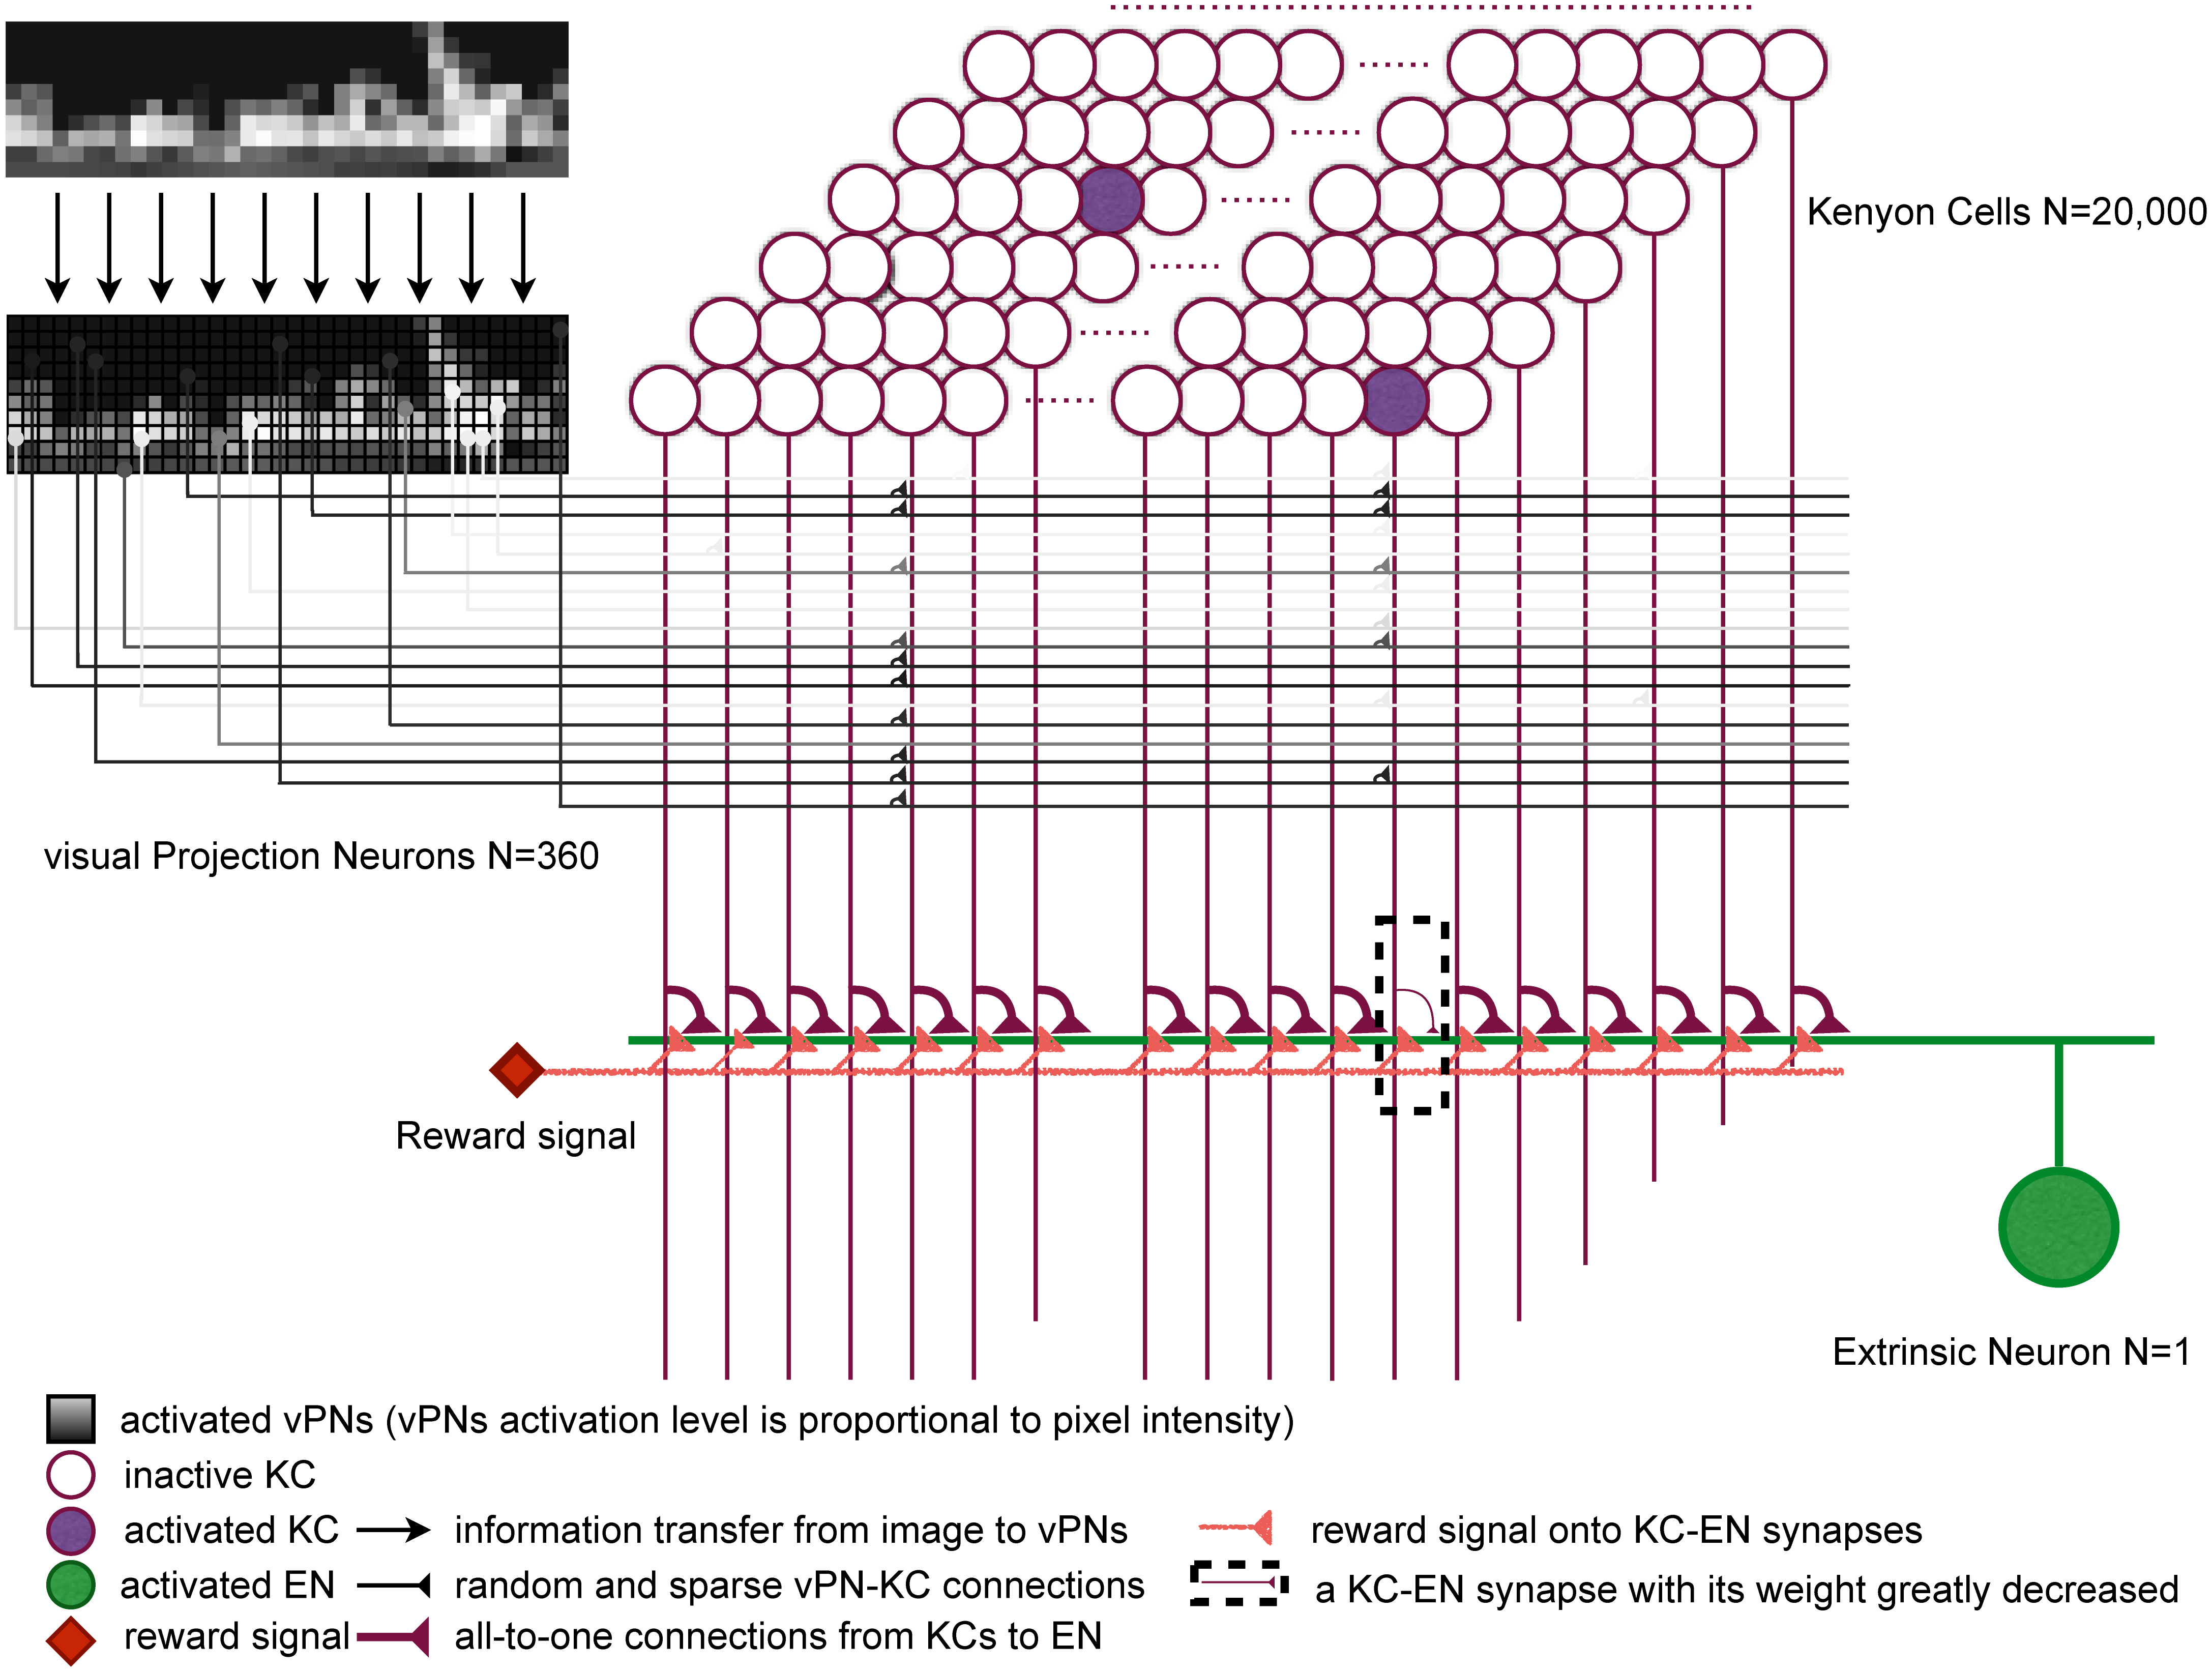
\includegraphics[width=0.7\textwidth]{Ardin2010MBModel}
  \caption{\label{fig:mb} The Mushroom Body circuit: (Caption from
    \textit{Ardin et al.}, Figure 2; note, their description and figure uses
    ``EN'' instead of ``MBON''): Images (see Fig 1) activate the visual
    projection neurons (vPNs). Each Kenyon cell (KC) receives input from 10
    (random) vPNs and exceeds firing threshold only for coincident activation
    from several vPNs, thus images are encoded as a sparse pattern of KC
    activation. All KCs converge on a single extrinsic neuron (EN) and if
    activation coincides with a reward signal, the connection strength is
    decreased. After training the EN output to previously rewarded (familiar)
    images is few or no spikes.}
\end{figure}

Learning occurs by showing patterns (images) to the vPNs. Each KC sums the
brightness of all connected vPNs and compares that sum to the activation
threshold. If the total brightness is greater than the threshold then the KC is
\textit{activated}. As the connections between the vPN and KC layers are random,
a given image will generate some sparse pattern of KC activation; to learn this
pattern, the weight of the KC-MBON connection is lowered from 1 to 0 for the
active KCs.
\newline
\par

To determine image familiarity during the recapitulation process, a pattern is
projected onto the vPNs (again giving a sparse pattern of KC activation).
The MBON then sums the synaptic (KC-MBON) weights of all active KCs to obtain a
\textit{familiarity} measure; recall, these weights are decayed as part of the
learing process; thus, the lower the MBON output, the more familiar the image
(and vice versa). Different route following strategies have been implemented
(scanning \cite{Ardin2016, Eberding2016, Zhang2017}, Klinokinesis
\cite{Zhang2017}, combination with the CX model \cite{Zhang2017}(see below), and
visual scanning \cite{Mitchell2018}); but, most commonly, some form of scanning
is used whereby the agent scans an arc for the most familiar direction.
\newline
\par

This has been a brief explanation for context. Part 1 gives slightly deeper
insight\cite{Mitchell2018} (particularly in relation to AntBot projects), and of
course the work of \textit{Ardin et al.} can give the full details
\cite{Ardin2016}.
\newline
\par

The MB model described above has been tested on the AntBot in three different
works (albeit using different methods and metrics); the network as presented in
\cite{Eberding2016, Zhang2017, Mitchell2018} differs only in the number of PNs
present (900 vPNs are used in all three works), and the KC
modelling (\textit{Ardin et al.} use a spiking model\footnote{The AntBot
  projects do not explicitly model membrane potentials and realistic responses.
  They use a simple abstraction for the sake of complexity. The network function
  is essentially the same.} for the KCs
\cite{Ardin2016}). More relevant to this work, is
the proposed modification given by \textit{Zhang}, whereby, 8 MBONs are present
as opposed to 1 (see Section \ref{CXMBBackground}).
\newline
\par

\subsection{ The Central Complex for Path Integration } \label{CXBackground}
The Central Complex (CX) is a highly conserved structure present in the insect
brain\cite{Pfeiffer2014, Stone2017}. Though the finer structural details and
component position may vary, the basic composition is more or less the same
across species \cite{Pfeiffer2014}. Organization and function of the
various parts of the CX are given by \textit{Pfeiffer and Homberg} in
\cite{Pfeiffer2014}\footnote{[DRAFT] I would like to include a short overview
  of the neurobiology but have left it until I can properly read through
  \cite{Pfeiffer2014}. I think I will need to leave this out, however, as I'm
  not sure how to summarise the most relevant parts of their work.
}
\newline
\par

We instead direct our attention to the CX model presented by
\textit{Stone et al.} which is the first neural model for path integration
in the insect brain, with structure drawn purely from physiology. Interestingly,
this model is a more advanced version of an earlier model presented by
\textit{Haferlach et al.}, which was \textit{evolved} using a Genetic Algorithm
\cite{Haferlach2007}. We present this also, purely for the sake of interest.

\subsubsection{The Evolved Model for Path Integration}
Prior to the CX model described below, there were several candidate neural
networks proposed for PI in ants \cite{Haferlach2007}. \textit{Haferlach et al.}
report the
two best-known candidates being hand-designed, with more recent research
into an evolutionary approach to network design \cite{Haferlach2007}. The
approach presented in \cite{Haferlach2007} follows this trend and employs
a Genetic Algorithm (GA) (see Appendix \ref{ap:ga} for a brief overview) to
evolve a neural model which is suitable for PI with biologically plausible
inputs.
\newline
\par

\textit{Haferlach et al.} encode solutions as lists of integers. In these lists
there are \textit{start markers} and \textit{end markers} which delimit
the definitions of the actual neurons or sensors present in the model. The
complete model (topography, connection weights, sensors, and effectors) is
limited to a fixed-size encoding (genome limited to 500 parameters; ~$50$ neurons
maximum) \cite{Haferlach2007}. An example encoding from \cite{Haferlach2007} can
be seen in Figure \ref{fig:markerbasedencoding}\footnote{[DRAFT] This figure
  doesn't seem to explain how the connections are actually mapped. A connection
  destination is given for the Sigmoid Neuron as +4 but I have no idea
  how this actually converts to a connection. Along the same lines, the
  Memory Neuron gives -6 as its connection destination, but it connects back
  to the Sigmoid Neuron which only required +4 to reach the Memory Neuron. How
  were these mappings determined?

  Glancing at the paper by \textit{Fullmer and Miikkulainen, 1992} (cited as
  inspiration); they give a key to each neuron which identifies it uniquely,
  which doesn't seem toappear in the model in the Figure
  \ref{fig:markerbasedencoding}.
}.
\newline
\par


\begin{figure}[h!]
  \centering
  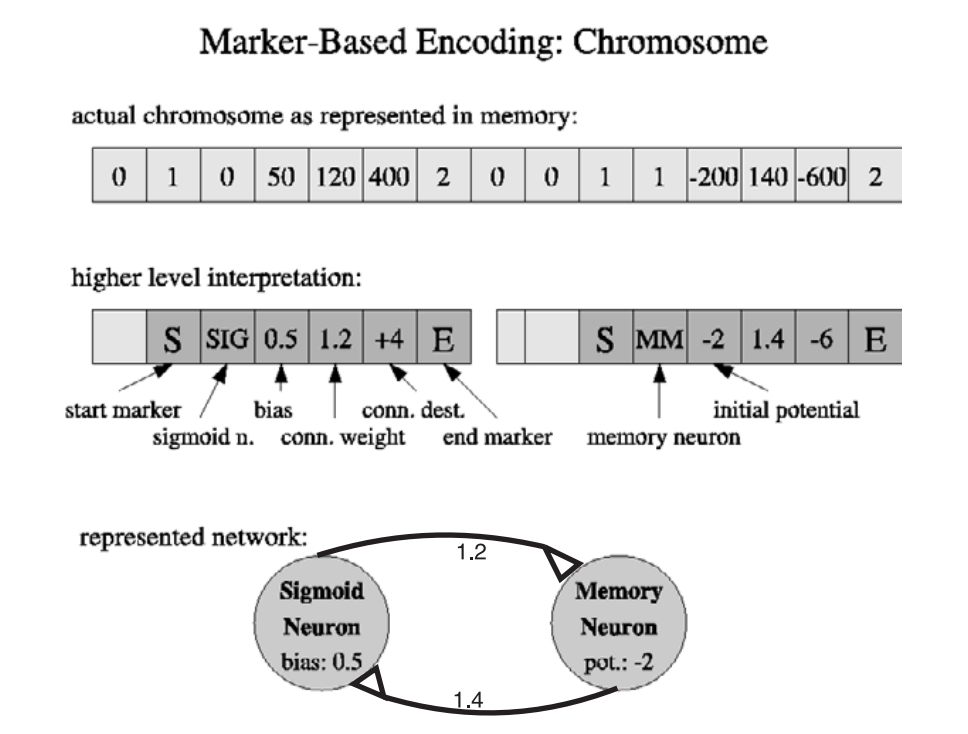
\includegraphics[width=0.9\textwidth]{MarkerBasedEncoding}
  \caption{\label{fig:markerbasedencoding} (Figure 2 from \cite{Haferlach2007})
    The Marker-Based encoding scheme used by \textit{Haferlach et al.},
    demonstrating how a simple neural model would be encoded as a sequence of
    integers.}
\end{figure}

Localised \textit{tournament selection}\footnote{Tournament Selection - Two
  solutions are picked randomly, then their fitness compared to determine if they
  will be selected} is used to pick solution for transition into the next
generation. Each solution is assigned a location in 1-dimensional space; a
solution is picked randomly, then another solution within distance $k$ of the
first is picked for the tournament ($k$ usually between 5 and 15)
\cite{Haferlach2007}. The solution with higher fitness wins the tournament
and progresses to mutation and \textit{crossover}\footnote{Crossover - A
  particular method for breeding two solutions whereby their genomes are cut at
  a particular point and the ends swapped.} This localised selection allows
the algorithm to find multiple \textit{good} solutions which need not share the
same genetic information.
\newline
\par

The fitness of each solution is evaluated by having the agent navigate an
outbound path through two randomly chosen points, then testing its ability
to navigate back to the start point. During the outbound phase, information is
input into the path integration network via the sensors; the network output is
ignored. During the inbound route, the agent is steered by the network output.
An individual is evaluated until some maximum time limit $m$ is reached, and the
distane to the start point $dist_t$ is computed at each time step. The fitness is
then the inverse sum of squared distances \cite{Haferlach2007}:

\begin{equation}
 f = \frac{1}{\sqrt{\int_{0}^m dist_t^2 dt}}
\end{equation}

The fitness is then augmented to penalise homeward routes which
spiral (circling the start point, getting closer with each pass), and
also to reward networks which are simple in structure; shown in
Equations \ref{eq:fithead} and \ref{eq:fitsimple} respectively\footnote{
  [DRAFT] I didn't have time to fix the equation formatting
  (equation number bumped out of position). This will be sorted
  in the final version.
  }.

\begin{multicols}{2}
  \begin{equation}
    \label{eq:fithead}
   f = \frac{1}{\sqrt{\int_{0}^m dist_t^2 |\theta - \omega | dt}}
  \end{equation}\break
  \begin{equation}
    \label{eq:fitsimple}
    f = \frac{1}{(1 + k_n)^{c_n}(1 + k_c)^{c_c}
      \sqrt{\int_{0}^m dist_t^2 |\theta - \omega | dt}}
  \end{equation}
\end{multicols}

where $\omega$ is the nest heading, $\theta$ is the agent's heading, $k_n$ is
a neuron penalty constant, $k_c$ is a connection penalty constant, $c_n$ is
the number of neurons, and $c_c$ is the number of connections (i.e.
the network is heavily penalised for the number of connections and neurons it
has, forcing simpler networks) \cite{Haferlach2007}. These are applied as a
two-stage evolutionary process; evolve a solution first using Equation
\ref{eq:fithead} to compute the fitness, then use this solution to seed a new
population and evolve a solution from here using Equation \ref{eq:fitsimple}. The
two-stage evolutionary processalone did not find acceptable solutions. The search
space was constrained by providing the following four constraints on network
topology: Each direction cell had to be connected to at least one memory neuron;
each direction cell had to be connected to at least one sigmoid neuron; sigmoid
neurons had to be connected to turn effectors; a maximum of two turn effectors
(left and right) were allowed \cite{Haferlach2007}.
\newline
\par

\textit{Haferlach et al.} present the model shown in Figure
\ref{fig:evolvednetwork}; notice the evolved structure bears a striking
resemblance to the CX model presented by \textit{Stone et al.} (Figure
\ref{fig:cx}). Indeed, this network operates on the same principle; encoding
a heading vector across multiple neurons with directional preference. This
network provides a compact, elegant, robust model capable of performing
path integration with reasonable errors. The network also demonstrated
some capability for PI with obstacles present (though errors were generally much
greater) \cite{Haferlach2007}.

\begin{figure}[h!]
  \centering
  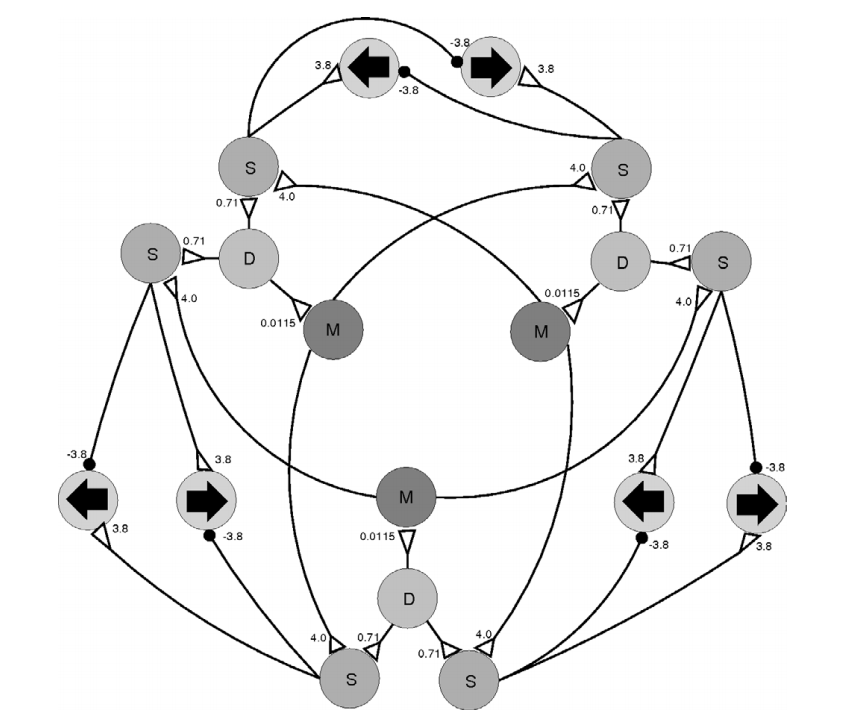
\includegraphics[width=0.7\textwidth]{EvolvedNetwork}
  \caption{\label{fig:evolvednetwork} (Figure 3 from \cite{Haferlach2007})
    The high-fitness network, consistently evolved using the constrained
    two-stage evolution process illustrated by \textit{Haferlach et al.}
  }
\end{figure}

\subsubsection{The Central Complex Model}
The Central Complex model is a six layer artificial neural network presented by
\textit{Stone et al.} which has been shown to provide a plausible neural
substrate for Path Integration (PI) both in simulation and on the AntBot platform
\cite{Scimeca2017, Stone2017}. The model presented is shown in Figure
\ref{fig:cx}. Splitting the model into its six layers, we get a breakdown of
functionality:
\newline
\par

\begin{itemize}
\item{Layer 1: Heading preprocessing (TL), Speed (TN)}
\item{Layer 2: Heading preprocessing (CL1)}
\item{Layer 3: Heading (TB1)}
\item{Layer 4: Memory (CPU4)}
\item{Layer 5: Normalisation and Inhibition (Pontine Neurons)}
\item{Layer 6: Steering/output (CPU1)}
\end{itemize}

\begin{figure}[h!]
  \centering
  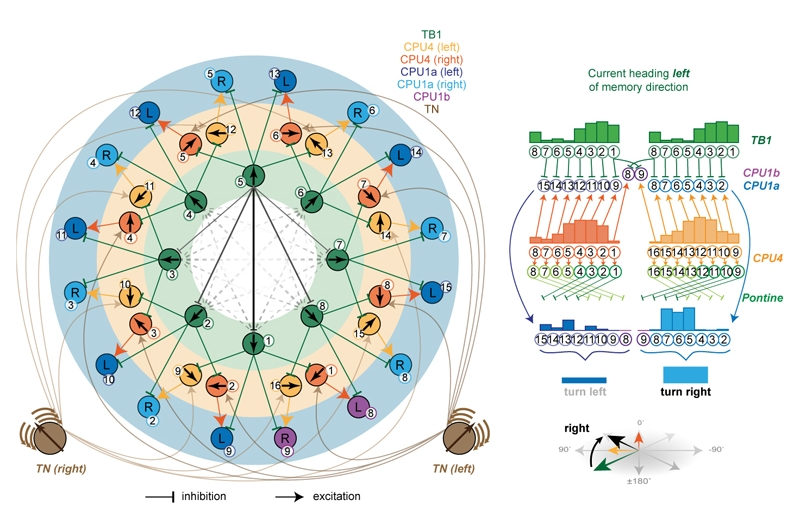
\includegraphics[width=\textwidth]{StoneCXModel}
  \caption{\label{fig:cx} The Central Complex model presented by
    \textit{Stone et al.}. (Left) This graph demonstrates the basic structure of
    the CX model (Figure 5G from \cite{Stone2017}). Pontine neurons have been
    excluded for clarity.
    (Right) This graph shows how signals propogate through the network where the
    current heading lies to the left of the desired heading, i.e. a right turn
    should be generated (Figure 5I from \cite{Stone2017}). The numbers given at
    each layer on the right correspond to the numbers given for each neuron
    in the graph on the left.
  }
\end{figure}

Figure \ref{fig:cx} shows four types of neuron: TN (Tangential Neuron), TB1
(green), CPU4 (yellow and orange), and CPU1 (dark blue, light blue, and purple).
\newline
\par

While Figure \ref{fig:cx} (Left) shows a distinction between CPU1a (blue) and
CPU1b (purple) neurons, we will ignore this distinction; for clarity, the
physiological mapping between these CPU1 subtypes in the Upper Central Body (CBU)
and the Protocerebral Bridge (PB) is different, but the function they serve in
the Central Complex is the same \cite{Stone2017}; thus, the distinction makes
no difference in the model. Similarly the normalisation and inhibition function
of the Pontine Neurons only has an effect when the agent experiences holonomic
motion (motion where the view direction does not match the direction of travel);
as AntBot is incapable of such motion, we can safely ignore the function of
the Pontine Neurons also; in our case, the Pontine Neurons would have the
same activity patterns as the CPU4 neurons \cite{Stone2017}. Figure \ref{fig:cx}
(Right) shows how the Pontine inhibition is structured.
\newline
\par

\begin{figure}[h!]
  \centering
  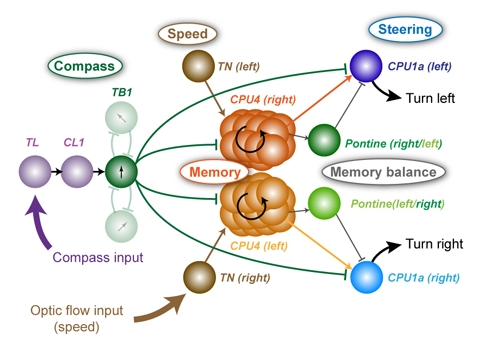
\includegraphics[width=0.7\textwidth]{Figure5F}
  \caption{
    \label{fig:cxlayer} Here we can see the layers of the CX model and
    how they fit together. A heading signal is input to the TL neurons,
    propogating through the CL layer to TB1 (heading ring-attractor) and
    CPU4 (memory). TN neurons (speed sensitivity) input directly to CPU4.
    So, the combination of heading and speed inputs to CPU4 gives a measure
    of distance travelled in a particular direction; this facilitates generation
    of a steering command in CPU1 providing a mechanism for Path Integration.
  }
\end{figure}

We now break down the different neuronal types and their proposed functions.
Citation is given, but for the avoidance of any doubt, the following descriptions
are adapted from \textit{Stone et al.} (see STAR Methods) \cite{Stone2017}.
We also add implementation information for the AntBot where appropriate;
occassionally the AntBot implementations are slightly different.
\newline
\par

\textbf{Simulated Neurons:}
Each neuron is described by its firing rate, where the firing rate $r$ is
a sigmoid function of the input $I$:

\begin{equation}
r = \frac{1}{1 + e^{-(aI - b)}}
\end{equation}

where $a$ and $b$ are parameters which control the slope and offset of the
sigmoid function \cite{Stone2017}. Optionally, Gaussian noise may be added
to the output. The input to each neuron is a weighted sum of the activity
of each neuron that synapses onto it; say neuron $j$, the input is:

\begin{equation}
  I_j = \sum_{i} w_{ij} \cdot r_i
\end{equation}

The weights used by \textit{Stone et al.} can only be 0, 1, or -1 for
no-connection, excitatory, or inhibitory respectively \cite{Stone2017}.
\newline
\par

% Function of CL & TL
\textbf{TL \& CL1:}
The TL neurons are the input point for heading information. In the ant brain
this heading information comes from a \textit{sky-compass}; the ant eye contains
cells sensitive to polarized light which allows the ant to infer an accurate,
allothetic direction from vision. Interestingly, there is also evidence that ants
have the capability to infer a direction without a view of celestial cues,
suggesting they may have access to some other signal, the candidate signal being
the geomagnetic field \cite{Fleischmann2018, Grob2017}. The TL neurons have been
shown to be polarisation sensiive across multiple insect species \cite{Stone2017}
(see STAR Methods). Each TL neuron has a preferred direction (i.e. a specific
direction of poliarisation sensitivity) $\theta_{TL} $, and there are 16 such
neurons representing the 8 directions around the agent (i.e.
$\theta_{TL} \in \{ 0^{\circ}, 45^{\circ}, 90^{\circ}, 135^{\circ}, 180^{\circ},
225^{\circ}, 270^{\circ}, 315^{\circ}\} $) \cite{Stone2017}. Together, the 16
TL neurons encode the heading of the agent in a single timestep; each neuron
receives input activation as:

\begin{equation}
  I_{TL} = cos( \theta_{TL} - \theta_{h} )
\end{equation}

where $\theta_{TL} $ is the preferred heading of the neuron as above, and
$\theta_{h} $ is the current heading of the agent. In the next heading layer,
there are 16 CL1 neurons which use inhibition to invert the polarisation
response \cite{Stone2017}. \textit{Stone et al.} comment that these neurons
effectively make no difference to the model and are included for completeness.
They are also included in previous AntBot projects which make use of the CX model
\cite{Zhang2017, Scimeca2017}. On AntBot, the heading is derived from the onboard
compass on the mobile phone (see Section \ref{sec:platform}).
\newline
\par

% Function of TN
\textbf{TN:}
There are 4 TN neurons which act as an input for speed information. The TN
neurons are sensitive to optical flow, and can be split into two subtypes:
TN1, and TN2. \textit{Stone et al.} showed that TN1 neurons are inhibited by
simulated forward flight and excited by simulated backward flight, while TN2
neurons are inhibited by simulated backward flight and excited by simulated
forward flight \cite{Stone2017}. Each of the four TN neurons has a tuning
preference; these tuning preferences were measured in bees as approximately
$+45^{\circ}$/$-45^{\circ}$ for TN2, and $+135^{\circ}$/$-135^{\circ}$ for TN1
(where $0^{\circ}$ is straight ahead). In short, we have TN$1_{left}$,
TN1$_{right}$, TN$2_{left}$, and TN$2_{right}$. It is thought that these neurons
provide a (or part of a) mechanism for odometry by allowing the model to
integrate speed with respect to time giving a distance measure \cite{Stone2017}.
\textit{Stone et al.} give the speed calculation from the TN neurons
as:

\begin{equation}
  I_{TN_{L}} =
  [ sin(\theta_{h} + \phi_{TN}) \quad cos(\theta_{h} + \phi_{TN}) ]\mathbf{v}
\end{equation}

\begin{equation}
  I_{TN_{R}} =
  [ sin(\theta_{h} - \phi_{TN}) \quad cos(\theta_{h} - \phi_{TN}) ]\mathbf{v}
\end{equation}

where $\mathbf{v}$ is the velocity of the agent in Cartesian coordinates,
$\theta_h \in [0^{\circ}, 360^{\circ})$ is the current heading of the agent, and
$\phi_{TN}$ is the preferred angle of that TN neuron \cite{Stone2017}.
\newline
\par

The TN neurons are not modelled in the \textit{basic} CX model on AntBot. There
is, however, a \textit{holonomic} implementation which models both the TN1 and
TN2 neurons is present on the robot. The formulae above are implemented on the
robot but they are never used. Instead, the raw left and right speeds computed
from the optical flow are passed in (see \textit{Scimeca} \cite{Scimeca2017} for
the details of speed computation from optic flow). The TN2 neurons will simply
clip these speeds to make sure they lie in $[0,1]$; the TN1 neurons will perform
$(1 - s) / 2$ for both the left and right speeds $s$, then clip the output to lie
in $[0,1]$. The output is returned directly, rather than being returned as a
sigmoid (as for all other neuron types).
\newline
\par

% Function of TB1
\textbf{TB1:}
There are eight TB1 neurons, each with a directional preference $\theta_{TB1}$,
which correspond to the eight cardinal directions in the model. Each TB1 neuron
receives excitatory input from the pair of CL1 neurons that have the same
directional preference. The TB1 layer contains inhibitory connections between
peer neurons where each TB1 neuron strongly inhibits other TB1 neurons with
opposite directional preferences (see Figure \ref{fig:cx}) forming a
\textit{ring attractor}\cite{Stone2017}. The weighting for an arbitrary
inhibitory connection from neuron $i$ to neuron $j$ is given by:

\begin{equation}
  w_{ij} =
  \frac{cos(\theta_{TB1,i} - \theta_{TB1,j}) - 1}{2}
\end{equation}

where $\theta_{TB1,i}$ is the direction preference of TB1 neuron $i$ (similarly
for $\theta_{TB1,j}$). The total input for each TB1 neuron from the CL1 layer
at timestep $t$ is:

\begin{equation}
  I_{TB1_{j}^{(t)}} =
  (1 - c) \cdot r_{CL1_j}^{(t)} + c \cdot \sum_{i = 1}^{8} w_{ij}
  \cdot r_{CL1_j}^{(t - 1)}
\end{equation}

where $c = 0.33$ is a scaling factor which determines the relative strength
of excitation from the CL1 layer and inhibition from other TB1 neurons;
the AntBot implementation of the TB1 neurons is the same. This
network layer produces a stable heading encoding which provides accurate
input for the CPU4 layer, underpinning accurate path integration.
\newline
\par

% Function of CPU4
\textbf{CPU4:}
The 16 CPU4 neurons receive input in the form of an accumulation of
heading $\theta_h^{(t)}$ of the agent, along with a modulated speed response
from the TN2 neurons \cite{Stone2017}. The CPU4 neurons accumulate distance with
direction. The input the CPU4 neurons is given by:

\begin{equation}
  \label{eq:cpu4update}
I_{CPU4}^{(t)} = I_{CPU4}^{(t - 1)} + h \cdot (r_{TN2}^{(t)} - r_{TB1}^{(t)} - k)
\end{equation}

where $h = 0.0025$ determines the rate of memory accumulation, and $k = 0.1$ is
a uniform rate of memory decay \cite{Stone2017}. All memory cells are initialised
to $I_{CPU4}^{(0)} = 0.5$ and are clipped at each timestep to fall between 0 and
1 \cite{Stone2017}. As shown in Figure \ref{fig:cx}, each TB1 provides input to
two CPU4 neuron, each of which receives input from the TN2 cell in the opposite
hemisphere. As these neurons accumulate distance with respect to a direction,
they provide a population encoding of the \textit{home vector} (the integrated
path back to the nest) \cite{Stone2017}. Interestingly, \textit{Zhang} showed
that the network can be initialised to an arbitrary state, allowing the agent
to navigate along arbitrary vectors \cite{Zhang2017}. While this seems intuitive,
the experimental evidence is valuable and demonstrates that the CPU4 layer could
form a basis for the \textit{vector memory} discussed by \textit{Webb} in
\cite{Webb2018} (see Section \ref{CXMBBackground}).
\newline
\par

The basic CX model on the AntBot does not model TN neurons, so the input is
computed differently; furthermore, the gain and loss factors are different.
The input can be expressed as:

\begin{align}
  I_{CPU4}^{(t)} =
  I_{CPU4}^{(t - 1)} + s \cdot ((1 - r_{TB1}^{(t)}) \cdot g - l)
\end{align}

where $l = 0.0026$ is the uniform rate of memory loss, $g = 0.005$ is the
uniform rate of memory gain, and $s$ is the current speed. This value is
then clipped to lie in $[0,1]$. As an aside, in the holonomic model
mentioned previously, the input is computed as in Equation \ref{eq:cpu4update}
as the TN neurons are present in the model.

\textbf{Pontine:}
The pontine neurons project contralaterally connecting opposite CBU columns
(shown in Figure \ref{fig:cx} (Right)). The 16 pontine neurons each receive input
from one CPU4 column \cite{Stone2017}; pontine input can be given simply as:
\newline
\par

\begin{equation}
  I_{Pontine}^{(t)} = r_{CPU4}^{(t)}
\end{equation}

The pontine neurons are not implemented on AntBot for simplicity. AntBot is
incapable of holonomic motion, so they would have no functional effect.
\newline
\par

% Function of CPU1
\textbf{CPU1:}
There are 16 CPU1 neurons present in the model. Each of which
receives inhibitory input (weight $= -1$) from a TB1 neuron; where, each
TB1 neuron provides inhibitory input to two CPU1 neurons (in the same pattern
as the TB1-CPU4 connections - see Figure \ref{fig:cx}). Each CPU4 neuron also
provides input to a CPU1 neuron (so we get input from vector memory and current
heading). The CPU1 input can be expressed as:

\begin{equation}
  I_{CPU1}^{(t)} = r_{CPU4}^{(t)} - r_{Pontine}^{(t)} - r_{TB1}^{(t)}
\end{equation}

As can be seen the CPU1 neurons also receive input from the pontine neurons.
The CPU1 neurons form two sets, those connecting to left motor units and those
connecting to the right. On AntBot the pontine term is omitted
(i.e. the input becomes
$I_{CPU1}^{(t)} = r_{CPU4}^{(t)} - r_{TB1}^{(t)}$).
\newline
\par

We choose a direction simply by summing the CPU1 outputs on both sides and the
difference indicates the direction and angle of the required heading correction:

\begin{equation}
  \theta_h^{(t)} = \theta_h^{(t - 1)} +
  m \cdot (\sum_{i = 1}^{8} r_{CPU1R_{i}} - \sum_{i = 1}^{8} r_{CPU1L_{i}})
\end{equation}

where $m = 0.5$ is a constant \cite{Stone2017}. The angle computation is the
same on the AntBot.
\newline
\par

There are some details which have been omitted for clarity. The stack presented
should effectively describe how the network generates a turning signal from its
current state and inputs to perform effective, accurate path integration. For
further details, please consult \cite{Stone2017} (the STAR Methods section
contains the full technical details of the model).

\subsection{ The Eight MBON Model (CXMB) } \label{CXMBBackground}
In \cite{Zhang2017}, the MB network is modified by adding 7 MBONs. Each MBON has
its own KC-MBON connection array, each with their own unique weights. Each
connection array corresponds to one of the eight cardinal directions represented
by the TB1 layer of the CX model (namely, $0^{\circ}$, $45^{\circ}$,
$90^{\circ}$, $135^{\circ}$, $180^{\circ}$ ,$225^{\circ}$, $270^{\circ}$,
$315^{\circ}$) (see Section \ref{CXBackground}).
\newline
\par

Image memory now has an associated direction, so, training is performed with
respect to orientation. For example, if the agent has a heading of $45^{\circ}$
when a image is stored, then only the corresponding connection array has its
weights updated during learning. Practically, this is done by querying the TB1
layer of the CX model to find the current direction according to the model
(rather than directly querying the robot's onboard compass). This process is
visualised in Figure \ref{fig:eightmbon}.
\newline
\par

\begin{figure}[h!]
  \centering
  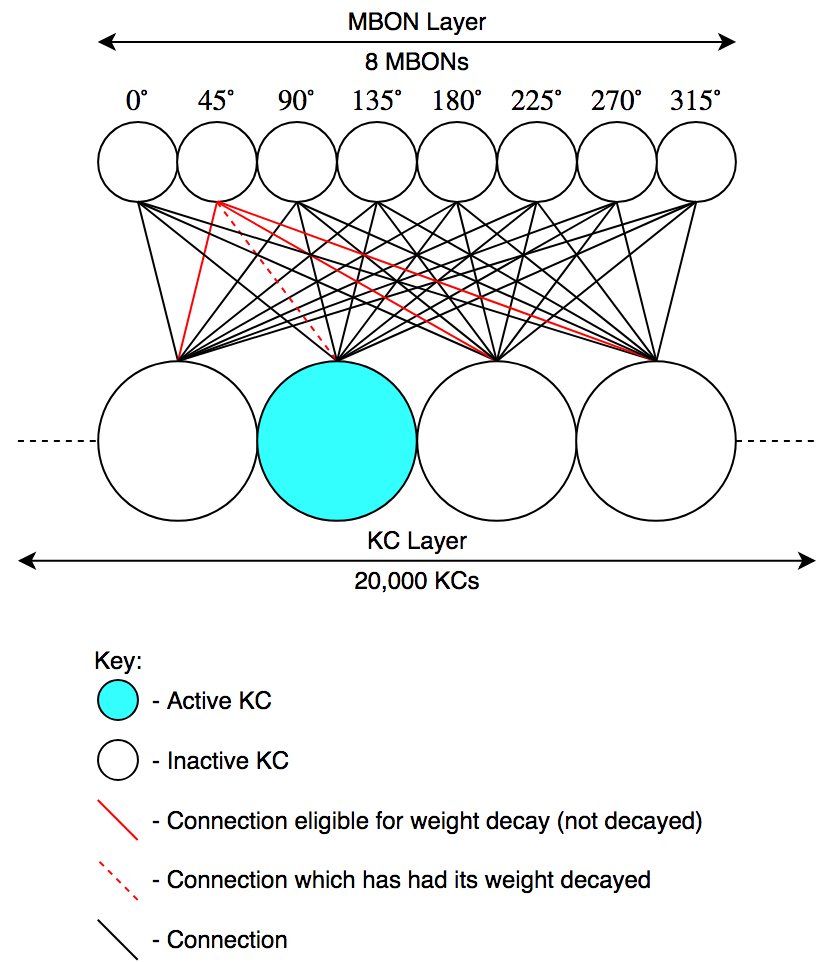
\includegraphics[width=0.9\textwidth]{EightENModel}
  \caption{\label{fig:eightmbon} Our interpretation of the eight MBON model
    proposed by \textit{Zhang}. Every KC connects to every MBON. All connection
    weights start out at $w=1$. Following the example presented in the text,
    if an image being learned corresponds to facing a direction of $45^{\circ}$,
    then only the conncetions to that MBON (highlighted in red) are eligible to
    have their weights modified. Recall, however, that these weights will only
    be modified if the KC was activated (not shown in the figure).
    }
\end{figure}

While, in theory, this eight MBON model could function independently,
\textit{Zhang} uses it to (rather neatly) augment the CX model; this allows
navigation to be performed using a combination of visual memory and path
integration information. The navigation process can be described by a sequence
of equations. We modify the notation slightly for clarity, but the
equations are the same as presented in \cite{Zhang2017}.
\newline
\par

The MB circuit is shown an image in the usual way; however, we now
get eight responses, giving us a response distribution. This distribution can
be interpreted as giving us the most likely direction of travel, when the image
presented was first observed. This distribution requires some modification to
integrate it into the CX response. Let $M_i$ be the familiarity response of the
$i$th MBON; the responses are normalised as:

\begin{equation}
  \bar{M}_i = \frac{M_i}{\Sigma^{8}_{k = 0} M_k}
\end{equation}

Which gives us the normalised response $\bar{M}_i$ between 0 and 1. $\bar{M}_i$
must be inverted so that the most likely direction has the greatest response
(in the MB model, the most familiar direction would give the lowest response):

\begin{equation}
  \bar{M}^{-1}_i = 1 - \bar{M}_i
\end{equation}

This visual response is then combined with the memory response from the CPU4
layer of the CX model to give output at the CPU1 layer:

\begin{equation}
  CPU1_{output} = k \cdot W_{CPU4} \cdot CPU4 + (1 - k) \cdot W_{MBON} \cdot
  \bar{M}^{-1}
\end{equation}

where $k$ is a weighting factor that determines the relative stregths of the CX
response and the MB response in the output ($k = 0.8$ in \cite{Zhang2017}),
$\bar{M}^{-1}$ is the collection of all inverse normalised MBON responses,
$W_{CPU4}$ is a custom matrix\footnote{This is the term used by \textit{Zhang} to
  describe   the $W_{CPU4}$ matrix. More specifically, this matrix describes the
  connections between the CPU4 and CPU1 layers of the CX model.}, $W_{MBON}$ is
an identity matrix that will expand the MBON response array from 8x1 to 16x1
\cite{Zhang2017}.
\newline
\par

In oreder to test the CXMB model, \textit{Zhang} first demonstrated the
functionality of a \textit{copied memory model}. The test of the copied memory
model aimed to prove that the CPU4 state of the agent could be copied and stored,
the CPU4 state modified, and then restored from the copy to allow the agent to
navigate home. The copied memory model was tested by sending the agent on a
pre-determined oubound route to a feeder (chosen at random, but consistent
between trials), copying the CPU4 state, and allowing the robot to navigate home
using the CX model; the CPU4 state will be modified by this homeward navigation.
The agent is then replaced at the feeder, its CPU4 state restored from the copy,
and tasked with navigating home a second time. The copied memory model was tested
as a pre-requisite for testing the CXMB model, however, it demonstrates an
important capability of the CX model; namely, the capability to directly load a
state into its memory in order to navigate; a concept referred to as
\textit{vector memory} in \cite{Webb2018}. Indeed, this concept of vector memory
is shown to be quite a useful tool in insect navigation \cite{Webb2018}. It is
worth noting that, the precise biological mechanism employed by insects to
perform this task, is unknown at time of writing. It would be neat to reuse
the CX circuitry, but this is an open question.
\newline
\par

The CXMB model is then tested in the same way. The agent follows its oubound
route to the feeder, navigates back once using the CX model (the MB model is
trained on this first inbound trip), is replaced at the
feeder, and finally, tasked with navigating back again, this time using the CXMB
model. To be clear, the CPU4 state of the CX model is stored after the outbound
route, and loaded back into the network before the second inbound trip.
\textit{Zhang} reports that the second inbound trip (using both CXMB) showed
more heading adjustments during its traversal, and, on average, performed
slightly better than a pure CX implementation\cite{Zhang2017}. It should also
be noted that the average performance of both models in \textit{Zhang's} work
was good \cite{Zhang2017}.
\newline
\par

We note two methodological problems with \textit{Zhang's} work: The outbound
route, while randomly chosen, was the same accross all trials, and, for the
copied memory and CXMB experiments, the agent was placed facing the nest for
the test run (second inbound). To add to the first problem, the outbound route
ended such that the robot was facing back towards the nest. Both of these flaws
could lead to apparent path integration behaviour where, in fact, the agent
could have made it sufficiently close to the nest by simply following a straight
line. While the agent was certainly employing the CX to perform path integration,
we do not feel that the tests chosen provide strong evidence of functionality.

\subsection{ Review of Part 1 }
The work in \cite{Mitchell2018} specifically covers the Mushroom Body
and Optical Flow Collision Avoidance. The Mushroom Body model used in
\cite{Mitchell2018} is the same as that used by \textit{Ardin et al.} in
\cite{Ardin2016}, except for the small differences noted in Section
\ref{MBBackground}. The model tested in \cite{Mitchell2018} used a single MBON
with a scan-based route following strategy. The scanning differed from previous
works as it was implemented as an image manipulation algorithm (termed
\textit{visual scanning}) instead of a physical turn performed by the AntBot.
\newline
\par

Multiple OFCA systems were tested, however, in final experiments an
optical flow filtering system is used. In short, a pattern of expected motion is
created, then the actual observed motion is projected on top of it. An absolute
difference is computed between the two and this can tell us if part of the image
is moving faster than we expect. This can be used to detect obstacles. This
strategy proved simple, but effective. While we move away from it for the
bulk of this project, it was used for initial tests of the CX model, as it
provided a simple out-of-the-box method to generate a non-deterministic
path for the model to integrate.
\newline
\par

Both systems functioned well and provided a solid baseline from which we will
work in this project. The MB model proved very capable at following routes
learned in a non-deterministic fashion through a cluttered environment.

\newpage

%%%%%%%%%%%%%%%%%%%%%%%%%%%%%%%%%%%%%%%%%%%%%%%%%%%%%%%%%%%%%%%%%%%%%%%%%%%%%%%
% PLATFORM                                                                    %
%%%%%%%%%%%%%%%%%%%%%%%%%%%%%%%%%%%%%%%%%%%%%%%%%%%%%%%%%%%%%%%%%%%%%%%%%%%%%%%
% High level description of the platform. This section can be short. Refer back
% to Part 1 for detail.
\section{ Platform } \label{sec:platform}
The AntBot is a small autonomous robot built to allow easy testing of the
various navigational algorithms in the \textit{Ant Navigational Toolkit}
on a physical agent. AntBot is assembled using off-the-shelf parts with an
Android phone at its heart. We give a high level description here; additional
detail can be found in \cite{Mitchell2018}.

\subsection{ Hardware }
The robot is composed of three main parts: a Dangu Rover 5 chassis, an Arduino,
and a Google Nexus 5 Android smartphone. The smartphone provides a
(theoretically) solid base for an autonomous agent, with sufficient processing
power and memory to run the models, a convenient touchscreen interface to display
information and an adaptable control interface, and a built-in camera and
extensive software libraries. As such, the smartphone works as the computational
centre, performing all higher sensory processing and acting on this analysis.
Once the algorithm running on the phone has decided on a course of action, it
sends a command via a serial connection to the Arduino board; the board, then
parses the command and translates it into a sequence of motor commands which are
sent to the built-in motor board in the chassis.
\begin{figure}
  \centering
  \includegraphics[width=0.7\textwidth]{AntBotCharging}
  \caption{
    \label{fig:antbotcomp} The AntBot, connected to the charging station.
    This figure also shows the position of the mobile phone, camera attachment,
    and retroflective motion capture markers on the top of the robot.
    }
\end{figure}

Additionally, the robot possesses a $360^{\circ}$ camera attachment, giving the
robot a panoramic view to match that of the desert ant\footnote{In reality,
  the desert ant has a visual field of only ~$280^{\circ}$\cite{Ardin2016},
  however an approxmiation of $360^{\circ}$ was considered appropriate when
  the robot was built.}. The robot was also modified as part of
\cite{Mitchell2018} to allow it to be charged with an external charger without
dismantling it.

\begin{figure}[t!]
  \centering
  \begin{minipage}[t!]{0.45\textwidth}
    \centering
    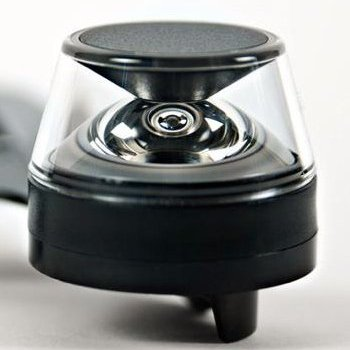
\includegraphics[width=0.9\textwidth]{KogetoDot}
    \caption{The Kogeto Dot 360$^\circ$ panoramic lens attachment.}
  \end{minipage}
  \hfill
  \begin{minipage}[t!]{0.45\textwidth}
    \centering
    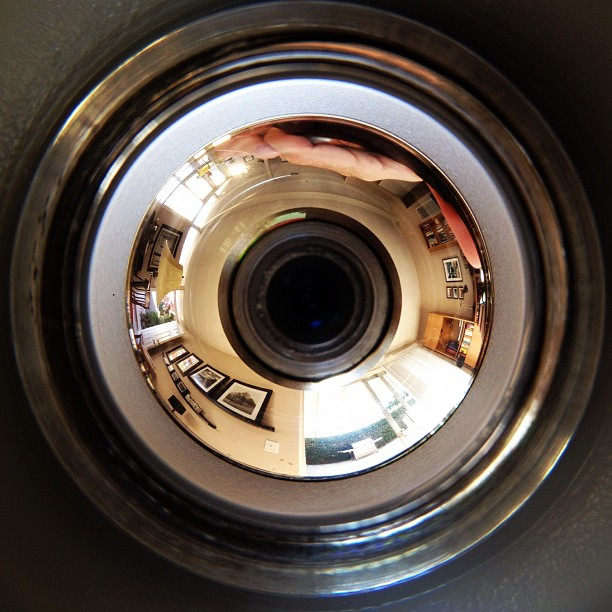
\includegraphics[width=0.9\textwidth]{PanoramicView}
    \caption{A sample view of the lens from the front facing camera, before any
      processing.}
  \end{minipage}

\end{figure}

\subsection{ Software }
The robot requires two levels of software; higher level Java (Android) code to
perform the high level functions; and, lower level code written in C/C++
(Arduino). The Arduino code can be thought of as the firmware.

\subsubsection{ Android } \label{subsubsec:droid}
Android can provide a nice basis for working on robotics projects. The
Operating System permts multiple applications to run asynchronously and
pass information between them; for example, the user could develop an application
to perform all visual processing then broadcast a processed image for other
applications which require it. The original AntBot software was split into
separate five applications: Ant Eye, Visual Navigation, Path Integration,
Combiner, and Serial Communications, neatly compartmentalising each task.
Unfortunately, in recent years, this structure was abandoned and almost all code
is contained within the \textit{AntEye} application. Only the Serial
Communications application remains true-to-design.
\newline
\par

Typical flow within AntEye will see an image captured from the front camera,
processed such that we get a downsampled 90x10 image which represents the
$360^{\circ}$ view around the robot. This image is then used for optical
flow analysis. The image and flow analysis are then made available to any thread
which requires it. A thread will then use this data to run an experiment.
\newline
\par

There are a lot of criticisms we can raise about the robot (in both a hardware
and software sense); ultimately the key problem may be lack of developer
familiarity with the Android platform.  While Android seems to work well at
first glance, it can ultimately be quite restrictive; we leave this to the
later discussion.

\subsubsection{ Arduino }
The Arduino code acts as a bridge between the Android platform and the Dangu
motor board, as there are no libraries which will directly connect the two.
The Android code contains a Command class which allows the user to insert robot
commands into the code; these are then transformed into serial messages by a
broadcast library \cite{Eberding2016} and sent to the Arduino. The Arduino code
contains a parser which will decode the serial messages and then call the
correct method to execute the desired motor commands.

\subsection{ Modifications and Development }
The modifications or additions listed below are a small part of the dissertation,
however, for one reason or another (see Discussion) these ended up taking
most of the project time. 

\textbf{Compass Sensor:}
While the Android phone has a built-in compass (used for other parts of this
project) this is impractical to use as part of a control system. The
communications delay is too great to allow accurate feedback control.
As a step to introducing proportional control to the robot, we undertook an
investigation into available compass sensors. Multiple sensors and libraries
were tested and ultimately we settled on a Grove 6-Axis Compass \& Accelerometer.
This sensor remained reasonably accurate in when tested alongside motors (a
source of magnetic interference) and the library code was straightforward to
include. The sensor was installed by the Informatics Workshop. While we have not
used it for this project, we would encourage a future student to make use of
this.
\newline
\par

\textbf{Ocular Calibration:}
The $360^{\circ}$ camera attachment is held in place by a pressure sensitive
adhesive which allows the position to shift if the attachment is knocked or
removed. The lens was removed for use in another project, and on re-attaching, it
was noticed that the image was warped, indicating that the pre-processing was not
working as required. The image pre-processing algorithm used a hard-coded pixel
value for the centre of the camera attachment which was no longer correct
(see Figure \ref{fig:centre}). We implemented a simple detection
algorithm using the Hough transform available in OpenCV to allow the user
to detect the new position of the camera attachment and set the centre
accordingly. The calibration is not performed automatically as the Hough
transform can be slow, and is highly dependent on lighting; instead, it
need only be done if the attachment is known to have moved.
\newline
\par


\begin{figure}
  \centering
  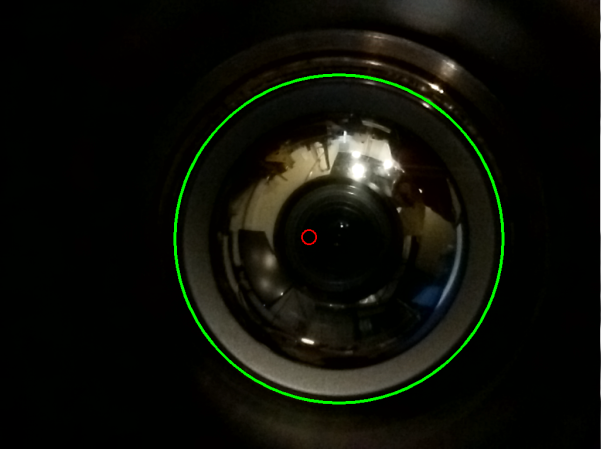
\includegraphics[width=0.7\textwidth]{Centre}
  \caption{\label{fig:centre} The hard-coded centre used for the polar transform
    (red), against the circle detected using the Hough transform (green).
   }
\end{figure}

\textbf{Code Refactor:}
As mentioned above, all behavioural code for the robot has moved into the AntEye
application. In fact, most code had been integrated into a single Android
Activity (Java Class); this file contained multiple long threads dictating
behaviour as well as a number of utility methods and robot commands. There
were also a ludicrous number of global variables. The resulting file was over
4000 lines long and almost unusable. Particuarly aggregious was the fact that
roughly half of the code was irrelevant to this project, but did need archived
for future use. As such, it was decided that it was worth refactoring the
codebase in order to make it easier to work. All utility functions were split
into their own static Util class, similarly, the robot control commands were
moved to the Command class. Runnable threads were moved into an archive
package, and split into classes according to their use: Mushroom Body,
Central Complex, Optical Flow, or Old Navigation; that final group consists of
the oldest code which is not used explicitly but is useful for reference
purposes. A single thread was left in the main Activity file to act as a test
thread. A lot of unused code was removed entirely.
\newline
\par

There are still many problems with the existing codebase. This simple refactor
ended up taking up a lot of time due to complications from working within the
Android framework; furthermore, many concessions had to be made for the same
reason.
\newline
\par

\textbf{Video Recording:}
In order to analyse the visual processing in more detail, a video recording
utility was added to AntBot. Again platform constraints mean that the utility
is perhaps not as well-made as it could be. A straightforward method using
FFMPEG had to be abandoned due to library conflicts; this method would
have allowed a video file to be recorded directly rather than the frame-stitching
solution described below. The real reason this proved difficult was that the
recording had to take place after preprocessing (image unwrapping and
downsampling to the 90x10 $360^{\circ}$ image). In order to achieve this frames
are passed off to a recording buffer after processing, the buffer is then
processed asynchronously by a separate thread which saves the frames to a
set directory. Pleasantly, this does not impact the frame rate. The video frames
then have to be retrieved from the robot and stitched together using a custom
python utility (a simple wrapper around an FFMPEG command). The recorded video
can then be analysed offline. This utility was created to offline analysis of
optical flow, however, it also highlighted a major problem with the robot which
was not previously known.
\newline
\par

\textbf{Video Pre-processing Pipeline:}
When stitching the video frames from the recorder, it was noticed that the
framerate was not quite right. The framerate on the robot was found to be
an unacceptably low 2fps. In an effort to improve the framerate we isolated
different parts of the processing pipeline. We found the best possible
framerate to be approximately 14fps with no processing (this is computed simply
as the numebr of times the \textit{onCameraFrame()} callback function is called
per-second). Adding processing steps back to the pipeline, two steps were found
which caused the framerate to crash. The first step was an image convolution
algorithm; the unwrapped image does not line up with the direction of travel of
the agent, so the resulting frame must be shifted (azimuth) so that the centre of
the frame is in line with the forward direction. This step was reducing the
framerate by approximately 5fps. Replacing the implemented algorithm with an
OpenCV library implementation reduced this to approximately 1fps cost. Similarly,
an image downsampling algorithm had been manually implemented which cost around
5fps; again, replacing this with an OpenCV library implementation reduced the
cost to approximately 1fps, if that. The full pipeline can now run at 10-12fps
with the recording utility running on top. When simulating a model like the ECX,
the framerate does drop to 8-10fps.
\newline
\par

This raises an interesting problem. We do not know when this code was added
to the robot but in any project following its insertion, the framerate surely
affected the performance of the agent. We can say for sure that the algorithms
used and tested in \cite{Mitchell2018} were affected. Indeed, in \cite{Mitchell2018}
it is noted that few images were stored during Visual Navigation experiments. The
low storage rate was thought to be a thread synchronisation issue, but it is now
clear that the frames were simply not finished processing in time to be stored.
In testing the matched-filter collision avoidance system from \cite{Mitchell2018}
we note a significant change in behaviour after the framerate improvement. It is
suspected that this is due to an increase in flow information, and therefore an
increase in noise which causes erroneous and erratic behaviour, not witnessed in
\cite{Mitchell2018}. 

\newpage

%%%%%%%%%%%%%%%%%%%%%%%%%%%%%%%%%%%%%%%%%%%%%%%%%%%%%%%%%%%%%%%%%%%%%%%%%%%%%%%
% METHODS                                                                     %
%%%%%%%%%%%%%%%%%%%%%%%%%%%%%%%%%%%%%%%%%%%%%%%%%%%%%%%%%%%%%%%%%%%%%%%%%%%%%%%
\section{ Methods } \label{sec:methods}
\textit{
  Methods not final, these are included as a rough plan/guide.
  }
\subsection{ Optical Flow }
% Discuss new method (eight directional FOEs)
\subsection{ Visual Navigation }
% Discuss directional recognition, as opposed to scanning.
\subsection{ Path Integration }
% Discuss CX implementation
\subsection{ The Complete System}

\section{Experimentation}\label{sec:test}
\textit{
  Experimentation methods not final, anything in this section illustrates a
  rough plan only.
}
\subsection{General}
\subsection{Collision Avoidance}
% Write new collision avoidance system, test it independently
\subsection{Visual Navigation}
% Do the same for the MB
\subsection{Path Integration}
% And for PI
\newpage

\section{ Results and Evaluation } \label{sec:results}
\textit{Included for skeleton purposes.}
\newpage

\section{ Discussion }
\textit{Included for skeleton purposes.}
\newpage

\bibliographystyle{plain}
\bibliography{working}
\appendix
\section{Genetic Algorithms} \label{ap:ga}
Genetic Algorithms (GAs) are metaheuristic
optimisation algorithms which aim to optimise some (arbitrary) objective
function. GAs perform this optimisation by taking inspiration from the
theory of evolution by natural selection wherein species advance by genetic
mixing (breeding) and a small chance of mutation with each offspring.
The theory of evolution by natural selection suggests that mutations
which are useful to the species become more potent over multiple generations
as they allow the individual to live longer and/or reproduce more than those
without the mutation; mutations which are useless die out or remain inert, and
those which are harmful tend not to survive. This is an extremely simplified
view.
\newline
\par

With appropriate representation, this evolutionary concept can be
translated into an optimisation algorithm. Say we choose to represent our data as
4-bit binary strings. To start with, we generate some population of $n$ random
4-bit bitstrings in the set range; two solutions are picked using some selection
process, usually based on \textit{fitness}\footnote{Fitness - some measure of how
  \textit{good} the solution is - e.g., minimisation would mean a lower value is
  fitter.} and ``breed'' with probability $p_c$; the offspring are then mutated
with (very small) probability $p_m$; finally the
offspring/mutant-offspring/original bitstrings \footnote{Note that those chosen
  may not breed with probability $p_c - 1$, and
similarly, they may not be mutated with probability $p_m - 1$} form the next
generation and the process repeats until some termination criterion is satisfied;
this could be time, number of generations, stagnation of the population, etc.
\newline
\par

This short explanation is merely to provide a high level idea of the concepts
employed when working with GAs; there is a great deal of depth and nuance
not captured by (and not necessary for) this paper. A tutorial by
\textit{Whitley} can be found in \textit{Statistics and Computing, Volume 4
  (1994)} \cite{Whitley1994}. Select terms will be defined as required.
\end{document}

